\chapter{Background}
\label{ch:background}

This chapter begins by introducing the foundational concepts of binary instrumentation within a Windows environment necessary to understand the proposed work. Subsequently, it analyzes state-of-the-art frameworks utilized for binary instrumentation. This overview is essential for contextualizing the compilation targets selected for our Domain-Specific Language (DSL), which are discussed in detail in \fullref{ch:method}.

\section{Windows Process Architecture and DLL Injection}

As discussed in \fullref{ch:introduction}, binary instrumentation allows us to change the runtime behavior of a binary. To achieve this in modern Windows environments, we must overcome several operating system constraints. Since every process operates within its own isolated virtual address space, a standard process cannot directly read or write the memory of another process. Therefore, to perform binary instrumentation, we must first find a way to inject and execute our custom instrumentation payload within the context (and memory space) of the target process. This is achieved through the use of \acp{DLL}.

While \acp{DLL} are traditionally used to share code libraries across multiple applications, they possess specific characteristics that make them the standard vehicle for Windows instrumentation:
\begin{enumerate}
	\item \textbf{Shared Address Space:} When a \ac{DLL} is loaded into a process, it is mapped directly into that process's virtual address space. This grants the \ac{DLL} full access to read, write, and patch the memory of the host process.
	\item \textbf{Automatic Initialization:} When a \ac{DLL} is successfully loaded, the Windows \ac{OS} loader automatically invokes its entry point function, \texttt{DllMain}. This allows the instrumentation framework to immediately execute its initialization sequence without requiring the host process to explicitly call any functions.
	\item \textbf{Automatic Cleaning:} If the \ac{DLL} is unloaded but the instrumentation code remains active in memory, subsequent executions will jump to an unmapped memory region, triggering an access violation. To ensure proper cleanup, when a \ac{DLL} is successfully unloaded, the Windows \ac{OS} loader automatically invokes its entry point function to execute the detachment logic.
	
	The following is the template code for an instrumentation DLL's entry point (\texttt{DllMain}):
	
	\begin{lstlisting}[language=C++, caption={DllMain code for attaching/detaching instrumentation}, label={lst:dllMain}, basicstyle=\ttfamily\footnotesize, breaklines=true]
		// Dll entry point
		BOOL APIENTRY DllMain (HMODULE hModule,
		  DWORD   ul_reason_for_call,
		  LPVOID  lpReserved)
		{
		  switch (ul_reason_for_call)
		  {
		    case DLL_PROCESS_ATTACH:
		      // Instrumentation framework-specific logic for injecting instrumentation
		      break;

		    case DLL_PROCESS_DETACH:
		      // Instrumentation framework-specific logic for disabling instrumentation
		      break;
		  }
			
		  return TRUE;
		}
	\end{lstlisting}
\end{enumerate}

To force a remote, unaware process to load our instrumentation \ac{DLL}, a technique known as \textbf{\ac{DLL} Injection} is utilized. The most common and reliable method relies on the Windows \ac{API} functions \texttt{CreateRemoteThread} and \texttt{LoadLibrary}. The injector process allocates memory in the target, writes the path of the \ac{DLL} into that memory, and spawns a thread (using \texttt{CreateRemoteThread}) pointing to \texttt{LoadLibrary}, which reads and processes the specified DLL path.

\section{The Application Binary Interface (ABI) and Calling Conventions}

Once the instrumentation \ac{DLL} is injected, it must interact with the target process's existing functions. To do this safely without corrupting the target process, the instrumentation framework must strictly adhere to the Application Binary Interface (ABI). The ABI defines the low-level rules for how functions interact at the assembly level, including how parameters are passed to a function, how return values are retrieved, and which entity is responsible for cleaning up the stack (the caller or the callee). These rules are formalized as \emph{Calling Conventions}.

In Windows x86 architectures, multiple calling conventions exist, such as:
\begin{itemize}
	\item \texttt{\_\_cdecl}: Arguments are pushed onto the stack from right to left, and the \emph{caller} cleans the stack.
	\item \texttt{\_\_stdcall}: The standard for the Windows \ac{API}. Arguments are pushed right to left, but the \emph{callee} cleans the stack.
	\item \texttt{\_\_fastcall}: The first two arguments are passed in the \texttt{ECX} and \texttt{EDX} registers for speed, while the rest are placed on the stack.
\end{itemize}

Understanding these conventions is critical for binary instrumentation. If an injected payload intercepts a \texttt{\_\_stdcall} function but is accidentally compiled as \texttt{\_\_cdecl}, the stack pointer will not be properly restored, leading to immediate memory corruption and process termination.

\section{Execution Context and CPU State Preservation}

Building upon the constraints of the \ac{ABI}, it is necessary to formally define what constitutes the execution context of a running process and why preserving it is paramount to process stability during any form of binary instrumentation. 

At any given nanosecond, the exact state of an executing thread is represented by the data held within the CPU's internal registers. On an x64 architecture, this includes General Purpose Registers, the Instruction Pointer, and various status flags (e.g., \texttt{EFLAGS}). Collectively, these transient values are referred to as the \emph{CPU state}.

When an instrumentation framework successfully intercepts the execution flow, it redirects the instruction pointer to the user's custom analysis payload. Because this payload is a compiled piece of software itself, it inevitably utilizes the CPU registers to perform its own calculations, memory allocations, or logging. This introduces a critical point of failure known as \textbf{register corruption}. If the custom payload overwrites the contents of a register that the original, interrupted application was actively using (for example, to store an intermediate loop counter or a critical memory pointer), that original data is permanently lost. 

When the payload finishes its execution and attempts to restore the original execution flow, the application will blindly continue operating using the corrupted register values. Therefore, to guarantee process stability, the original CPU state must be flawlessly preserved by the instrumentation framework.

\section{Paradigms of Binary Instrumentation}

Modern instrumentation engines generally fall into two broad architectural paradigms:
\begin{itemize}
	\item \textbf{Inline API Hooking:} this paradigm involves modifying the original execution flow via localized jumps. It patches specific functions in memory, redirecting execution to a custom payload before returning to the original flow.
	\item \textbf{Dynamic Binary Instrumentation (\ac{DBI}):} rather than modifying the original binary in place, \ac{DBI} engines physically copy, recompile, and execute instructions inside a localized sandbox known as a Code Cache.
\end{itemize}

\section{Inline API Hooking Architectures}

Hooking is the specific mechanism used to instrument a function. A hook allows the redirection of the execution flow from the original code to newly injected analysis code. A standard inline hook consists of three primary logical components:
\begin{enumerate}
	\item \textbf{The Target:} the original function whose execution we wish to intercept. The goal is to patch the first 5 to 7 bytes of the target function with an unconditional jump (\texttt{JMP}) to a user-defined payload. These initial bytes are restored to the target function once the instrumentation is complete and the framework detaches from the host process.
	\item \textbf{The Detour (or Payload):} the custom function injected by the instrumentation framework. This function receives the execution flow, inspects the target function's arguments or return value, performs the desired analysis or policy enforcement, and then dictates whether the execution should continue or be blocked.
	\item \textbf{The Trampoline:} in the paradigm of inline API hooking, placing an interception branch (\texttt{JMP}) inherently corrupts the target function's prologue. To maintain execution continuity, all inline instrumentation frameworks must implement an Out-of-Line Execution Bridge, universally referred to as a \textbf{``Trampoline''}. Conceptually, the trampoline is a dynamically allocated, executable memory buffer that fulfills two architectural mandates: it securely relocates the displaced prologue instructions and unconditionally routes the instruction pointer back to the unpatched remainder of the target function.
\end{enumerate}

The manner in which these frameworks handle the CPU state and the \ac{ABI} constraints defines their underlying architecture.

\subsection{Bare-Metal Hooking: Microsoft Detours and MinHook}
Frameworks like Microsoft Detours and MinHook are specifically designed for Windows x86/x64 and utilize a \textbf{``bare-metal'' routing} approach. In this model, the hooking library has zero awareness of the CPU state or context at runtime. Consequently, they strictly enforce the \ac{ABI}. The developer must possess precise knowledge of the C/C++ signatures (argument types and return types) and calling conventions of the function being hooked. As shown in \Cref{lst:detours}, using these two frameworks requires a strict type definition of the target function pointer to avoid stack corruption:



\begin{lstlisting}[language=C++, caption={Detours/MinHook requires strict ABI compliance.}, label={lst:detours}, basicstyle=\ttfamily\footnotesize, breaklines=true]
		// Strict function pointer definition required by Detours
		static int (WINAPI * TrueMessageBoxW)(HWND, LPCWSTR, LPCWSTR, UINT) = MessageBoxW;
		
		// Strict function pointer definition required by MinHook
		typedef int (WINAPI * MESSAGEBOXW)(HWND, LPCWSTR, LPCWSTR, UINT);
		MESSAGEBOXW fpMessageBoxW = NULL;
	\end{lstlisting}

Furthermore, to access the arguments correctly, the hooked version of the function must strictly adhere to the original signature:

\begin{lstlisting}[language=C++, caption={Strict ABI compliance even in the Hooked Function}, label={lst:detours2}, basicstyle=\ttfamily\footnotesize, breaklines=true]
		// Detours (same for MinHook)
		int WINAPI HookedMessageBoxW(HWND hWnd, LPCWSTR lpText, LPCWSTR lpCaption, UINT uType)
	\end{lstlisting}

Following these guidelines ensures the compiler generates the correct code to prevent stack and register corruption and to correctly access the arguments of the target function being monitored or modified.

The code structure for the hooked function is identical in both frameworks. In the following example, the goal is to intercept a target process's call to \texttt{MessageBoxW} and modify the displayed dialog with custom text (\texttt{customCaption}) and altered options (\texttt{modifiedType}) during the PRE-LOGIC phase. After this, the trampoline is called, the original function is executed with the modified arguments, and control is returned to the hooked version (POST-LOGIC). Here, we intercept the user's choice (\texttt{result}), forcing a "yes" outcome even if the user pressed "no", and return the final result to the target process:

\begin{lstlisting}[language=C++, caption={Detours/MinHook Hooked function structure}, label={lst:detours3}, basicstyle=\ttfamily\footnotesize, breaklines=true]
		// Detours (same for MinHook)
		int WINAPI HookedMessageBoxW(HWND hWnd, LPCWSTR lpText, LPCWSTR lpCaption, UINT uType)
		{
		  // PRE-LOGIC
		  UINT modifiedType = MB_YESNO;
		  LPCWSTR customCaption = L"Hooked! Please choose:";
		  
		  // Call to the trampoline
		  int result = TrueMessageBoxW(hWnd, lpText, customCaption, modifiedType);
		  
		  // POST-LOGIC
		  if (result == IDNO) 
		  {
		    std::cout << "[HOOK POST-LOGIC] Intercepted IDNO (No). Changing result to IDYES (Yes)!" << std::endl;
		    result = IDYES; 
		  }
		  else if (result == IDYES)
		  {
		    std::cout << "[HOOK POST-LOGIC] Intercepted IDYES (Yes). Nothing to do." << std::endl;
		  }
		  
		  return result;
		}
	\end{lstlisting}

\subsection{Context-Aware Routing: Frida-Gum}
Frida-Gum is the underlying C library of the Frida instrumentation toolkit, representing a modern approach to cross-platform instrumentation (X86/X64, ARM/ARM64, MIPS). In contrast to bare-metal routing, Frida-Gum utilizes \textbf{``Context-Aware Routing.''} When a hook is triggered, the framework jumps not directly to the custom payload, but into a dynamically allocated memory block containing instructions that save all CPU registers into a hardware-agnostic structure (\texttt{GumInvocationContext}) before invoking the payload. After the hooking callbacks execute, these saved values are used to restore the CPU state exactly as it was prior to the hook, preventing process crashes.

This context awareness normalizes the \ac{ABI} and abstracts the target process architecture. The developer does not need to define strict C++ function signatures; arguments and return values are accessed and modified dynamically by their index, regardless of the target process architecture. Due to these architectural differences, the implementation significantly diverges from that of Detours and MinHook. The developer only needs to specify the \texttt{on\_enter} and \texttt{on\_leave} hooking callbacks: \texttt{on\_enter} executes before the target function, while \texttt{on\_leave} executes after it finishes. 

Below is the Frida-Gum equivalent code for altering the behavior of \texttt{MessageBoxW}:

\begin{lstlisting}[language=C, caption={Frida-Gum \texttt{on\_enter}/\texttt{on\_leave} for hooking MessageBoxW.}, label={lst:frida}, basicstyle=\ttfamily\footnotesize, breaklines=true]
		// Pre-logic
		static void
		example_listener_on_enter (GumInvocationContext * ic,
		  gpointer user_data)
		{
		  // The arguments for MessageBoxW are 0-indexed:
		  // 0: HWND hWnd
		  // 1: LPCWSTR lpText
		  // 2: LPCWSTR lpCaption
		  // 3: UINT uType
		  
		  // Frida-Gum allows contextual argument extraction without strict C signatures
		  guint originalType = GPOINTER_TO_UINT (gum_invocation_context_get_nth_argument (ic, 3));
		  guint modifiedType = MB_YESNO;
		  
		  static const wchar_t* customCaption = L"Hooked, choose:";
		  
		  gum_invocation_context_replace_nth_argument (ic, 2, (gpointer) customCaption);
		  gum_invocation_context_replace_nth_argument (ic, 3, GUINT_TO_POINTER (modifiedType));
		}
		
		// Post-logic
		static void
		example_listener_on_leave (GumInvocationContext * ic,
		  gpointer user_data)
		{
		  int result = GPOINTER_TO_INT (gum_invocation_context_get_return_value (ic));
		  
		  if (result == IDNO) 
		  {
		    g_print ("Intercepted IDNO (No). Changing result to IDYES (Yes)\n");
		    gum_invocation_context_replace_return_value (ic, GINT_TO_POINTER (IDYES));
		  }
		  else if (result == IDYES)
		  {
		    g_print ("Intercepted IDYES (Yes). Nothing to do\n");
		  }
		}
	\end{lstlisting}

\subsection{Passive vs. Active Trampoline Architectures}

While all the presented frameworks utilize inline prologue patching, their trampoline architectures are fundamentally opposed. Detours and MinHook utilize a \textbf{Passive Trampoline}, strictly acting as a repository for displaced instructions and forcing the user's hook to act as the primary execution controller (the developer's C++ code manually calls the Trampoline). 
Conversely, Frida-Gum utilizes an \textbf{Active Trampoline}: when the target function is intercepted, execution jumps directly into the trampoline, which assumes total control of execution routing and register preservation, as depicted in \Cref{fig:instrumentation_comparison}:

\begin{figure}[H]
	\centering
	
	\begin{subfigure}{0.6\textwidth}
		\centering
		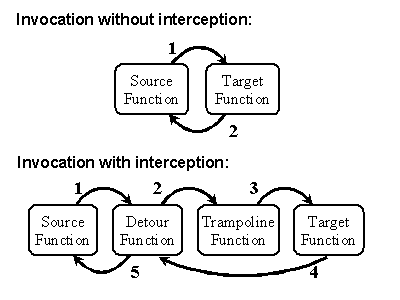
\includegraphics[width=\textwidth]{images/Detours_ovr_Technical_Figure_1.png}
		\caption{Detour/MinHook Execution Flow}
		\label{fig:Det}
	\end{subfigure}
	
	\vspace{1em} % Add some vertical space between the stacked images
	
	\begin{subfigure}{0.98\textwidth}
		\centering
		\includegraphics[width=\textwidth]{images/frida_flow.png}
		\caption{Frida-Gum Execution Flow}
		\label{fig:Frida}
	\end{subfigure}
	
	\caption{A comparison between the different architectures and roles of the Trampoline}
	\label{fig:instrumentation_comparison}
\end{figure}

\subsection{Instruction Boundaries and the Role of Disassemblers}

\note{Advisor}{cyan}{Non so se mettere questa sezione}
A fundamental challenge in implementing the hook structure described above, particularly on Intel x86 and x64 architectures, is the variable-length nature of the instruction set. To detour a target function, an inline hooking framework typically needs to overwrite the first few bytes of the function's prologue with an unconditional jump (\texttt{JMP}) to the custom payload. In a standard 32-bit architecture, this jump requires 5 bytes (1 byte for the opcode, 4 bytes for the relative address).

If the framework blindly overwrites exactly 5 bytes, it risks cutting an existing instruction in half. For example, if the original prologue consists of two 3-byte instructions, overwriting 5 bytes will corrupt the second instruction, leaving a hanging, invalid byte. When the trampoline attempts to execute these copied bytes to resume the program, the CPU will encounter an invalid opcode and crash the process.

To prevent this, hooking frameworks must incorporate a Length Disassembler Engine (LDE). Before applying any patches, the engine disassembles the target function's prologue to calculate exact instruction boundaries. It then copies whole, unfragmented instructions into the trampoline until it has safely relocated at least the number of bytes required for the jump (padding any remaining bytes in the original function with \texttt{NOP} instructions).

The choice of disassembler heavily impacts the footprint and dependencies of the framework:
\begin{itemize}
	\item \textbf{Microsoft Detours} relies on a proprietary, internal instruction decoder optimized specifically for standard compiler prologues.
	\item \textbf{MinHook} utilizes a highly optimized, custom-built Hacker Disassembler Engine (HDE32/HDE64), as it only needs to calculate instruction lengths rather than fully analyze instruction semantics.
	\item \textbf{Frida-Gum} requires deep semantic analysis of the instructions to achieve its context-aware routing. To accomplish this, it statically links against Capstone, a comprehensive and heavy multi-architecture disassembly framework, significantly increasing the size of the resulting \ac{DLL}.
\end{itemize}

\subsection{Transactional Patching: Safe Attachment and Detachment}

Another critical challenge in inline hooking is applying the memory patch (e.g., the \texttt{JMP} instruction) to a live, running process without causing a \textbf{race condition}. 
In a multi-threaded application, if one thread attempts to execute a target function at the exact moment the instrumentation framework is overwriting its prologue, the CPU may attempt to execute a partially written, invalid instruction.

To guarantee thread safety during the patching phase (both attaching and detaching), modern instrumentation frameworks implement a \textbf{transactional model}. Instead of patching memory directly and immediately, the developer queues the hooks. When the transaction is finalized, the framework briefly suspends all threads in the target process (except the one applying the patch), writes the bytes to memory atomically, flushes the CPU's Instruction Cache, and finally resumes the suspended threads.

\textbf{Detours} makes this transaction explicitly visible to the developer. The \ac{API} requires opening a transaction, manually declaring which threads need to be stopped, attaching/detaching the specified hooks, and committing the transaction:

\begin{lstlisting}[language=C++, caption={Microsoft Detours transactional model for safe attachment and detachment.}, label={lst:detours_lifecycle}, basicstyle=\ttfamily\footnotesize, breaklines=true]
		// --- SAFE ATTACHMENT ---
		// Start the transaction
		DetourTransactionBegin();
		
		// Enlist threads to be suspended during the patch
		DetourUpdateThread(GetCurrentThread()); 
		// here we specify possible other threads we want to stop...
		
		// Queue the hooks
		DetourAttach(&(PVOID&)TrueMessageBoxW, HookedMessageBoxW);
		// here we specify possible other hooks we want to inject...
		
		// Apply patches atomically, suspending the specified threads and flushing the instruction cache
		DetourTransactionCommit();
		
		
		// --- SAFE DETACHMENT ---
		DetourTransactionBegin();
		
		DetourUpdateThread(GetCurrentThread());
		// here we specify possible other threads we want to stop...
		
		DetourDetach(&(PVOID&)TrueMessageBoxW, HookedMessageBoxW); // Queue removal
		// here we specify possible other hooks we want to detach...
		
		DetourTransactionCommit();
		// Suspends threads, restores original bytes, resumes
	\end{lstlisting}

\textbf{MinHook} abstracts the explicit transaction start and end calls, but enforces the exact same synchronization internally when hooks are enabled or disabled (\Cref{lst:minhook_lifecycle}):

\begin{lstlisting}[language=C++, caption={MinHook internal thread synchronization during enable/disable phases.}, label={lst:minhook_lifecycle}, basicstyle=\ttfamily\footnotesize, breaklines=true]
		// --- SAFE ATTACHMENT ---
		MH_CreateHook(&MessageBoxW, &HookedMessageBoxW, reinterpret_cast<LPVOID*>(&fpMessageBoxW));
		// here we specify possible other hooks we want to inject...
		
		// MH_EnableHook internally suspends threads, writes the JMP, and resumes
		MH_EnableHook(&MessageBoxW);
		//or MH_EnableHook(MH_ALL_HOOKS); if we have more than one hook
		
		// --- SAFE DETACHMENT ---
		// MH_DisableHook internally suspends threads, restores original bytes, and resumes
		MH_DisableHook(&MessageBoxW);
		//or MH_DisableHook(MH_ALL_HOOKS); if we have more than one hook
	\end{lstlisting}

\textbf{Frida-Gum} employs an identical safety mechanism through its Interceptor \ac{API}:

\begin{lstlisting}[language=C, caption={Frida-Gum utilizing transaction boundaries for hook management.}, label={lst:frida_lifecycle}, basicstyle=\ttfamily\footnotesize, breaklines=true]
		// --- SAFE ATTACHMENT ---
		gum_interceptor_begin_transaction (interceptor);
		
		gum_interceptor_attach (interceptor,
		  GSIZE_TO_POINTER (gum_module_find_export_by_name (user32, "MessageBoxW")),
		  listener,
		  NULL,
		  GUM_ATTACH_FLAGS_NONE);
		// here we specify possible other hooks we want to inject...
		
		gum_interceptor_end_transaction (interceptor);
		// Threads are paused and patches applied
		
		// --- SAFE DETACHMENT ---
		gum_interceptor_begin_transaction (interceptor);
		
		gum_interceptor_detach (interceptor, listener);
		// here we specify possible other hooks we want to detach...
		
		gum_interceptor_end_transaction (interceptor);
		// Threads are paused and bytes restored
	\end{lstlisting}

\section{Dynamic Binary Instrumentation (\ac{DBI}) Architectures}

For deeper execution analysis at the assembly level, \ac{DBI} engines are utilized. Unlike inline hooking, which patches the original binary in place, \ac{DBI} engines ensure that the target application's original code is never executed directly by the CPU. Instead, the framework employs a \textbf{Just-In-Time (JIT) compilation} mechanism to dynamically translate and instrument instruction sequences.

\subsection{Core Architectural Components}
Modern \ac{DBI} frameworks rely on a unified architectural pattern comprising the following components:

\begin{description}
	\item[1. The Dispatcher (Control Flow Manager):] The dispatcher is the central component of the \ac{DBI} engine, responsible for orchestrating the execution state. Because the application and the \ac{DBI} framework share the same process but operate under different scopes, they must safely transit between ``framework mode" and ``application mode." The dispatcher trigger a context-switch mechanism that carefully saves and restores the application's state whenever execution exits or enters the code cache.
	\item[2. \ac{JIT} Compiler:] Instead of translating the entire binary before execution, these architectures translate the application's instructions dynamically in small fragments. During this translation phase, the framework decodes and encodes (into the framework's abstraction) the original instructions and has the opportunity to insert custom instrumentation code or patches before emitting the new sequence.
	\item[3. The Code Cache (The Execution Sandbox):] To mitigate the massive performance penalty of repeatedly translating the same code, \ac{DBI} frameworks employ a software-based code cache. The translated and potentially instrumented fragments are stored in this sandboxed memory region. When the application re-executes a previously translated section of code, it runs directly from the code cache, which significantly optimizes execution speed.
	\item[4. The Client Interface (Instrumentation API):] This is the abstraction layer exposed to the developer. It provides the necessary functions to inspect the program state, traverse instruction sequences, and specify exactly where and how instrumentation should be injected.
\end{description}

\subsection{The Execution Lifecycle: The JIT Loop}
To formally describe how these components interact at runtime, we can outline the execution lifecycle of a standard block of code:

\begin{enumerate}
	\item \textbf{Interception:} The target application attempts to execute a block of original code. The \ac{DBI} engine intercepts this attempt and yields control to the Dispatcher.
	\item \textbf{Cache Lookup:} The Dispatcher queries a fast-lookup hash table to check if the target memory address has already been translated. If it results in a cache hit, the CPU is redirected to the Code Cache.
	\item \textbf{Translation (On Cache Miss):} If the code has not been encountered before, the \ac{JIT} Compiler decodes original binary instructions one by one to form a straight-line sequence that terminates at a control transfer, such as a branch, call, or return.
	\item \textbf{Instrumentation:} The engine queries the Client Interface to determine if the user wishes to instrument the block or a single instruction within it. If so, the instrumentation instructions are injected. 
	\item \textbf{Emission and Linking:} Most \ac{DBI} frameworks use this phase to apply patches to the control-flow instructions at the end of the sequence, guaranteeing that when the block finishes running, it will redirect back to the framework rather than jumping to a native memory address. If the block ends in a direct branch to another previously translated block, the engine ``links'' them together directly in the cache (if it was an indirect branch, it cannot know the target before executing it), allowing the CPU to bypass the Dispatcher in future iterations. The modified block is emitted into the Code Cache.
	\item \textbf{Execution:} The Dispatcher performs a context switch, restoring the application state, and commands the CPU to execute the newly cached block natively.
	\item \textbf{Code Cache Exit:} Execution remains safely inside the code cache --- often jumping directly from one translated block to another through ``linking''---until it hits a boundary. This boundary might be an unlinked branch or an indirect branch whose target hasn't been translated yet. When this happens, the block executes an exit stub which saves the CPU's state and transfers control back to the Dispatcher, restarting the loop.
\end{enumerate}

\begin{figure}[H]
	\centering
	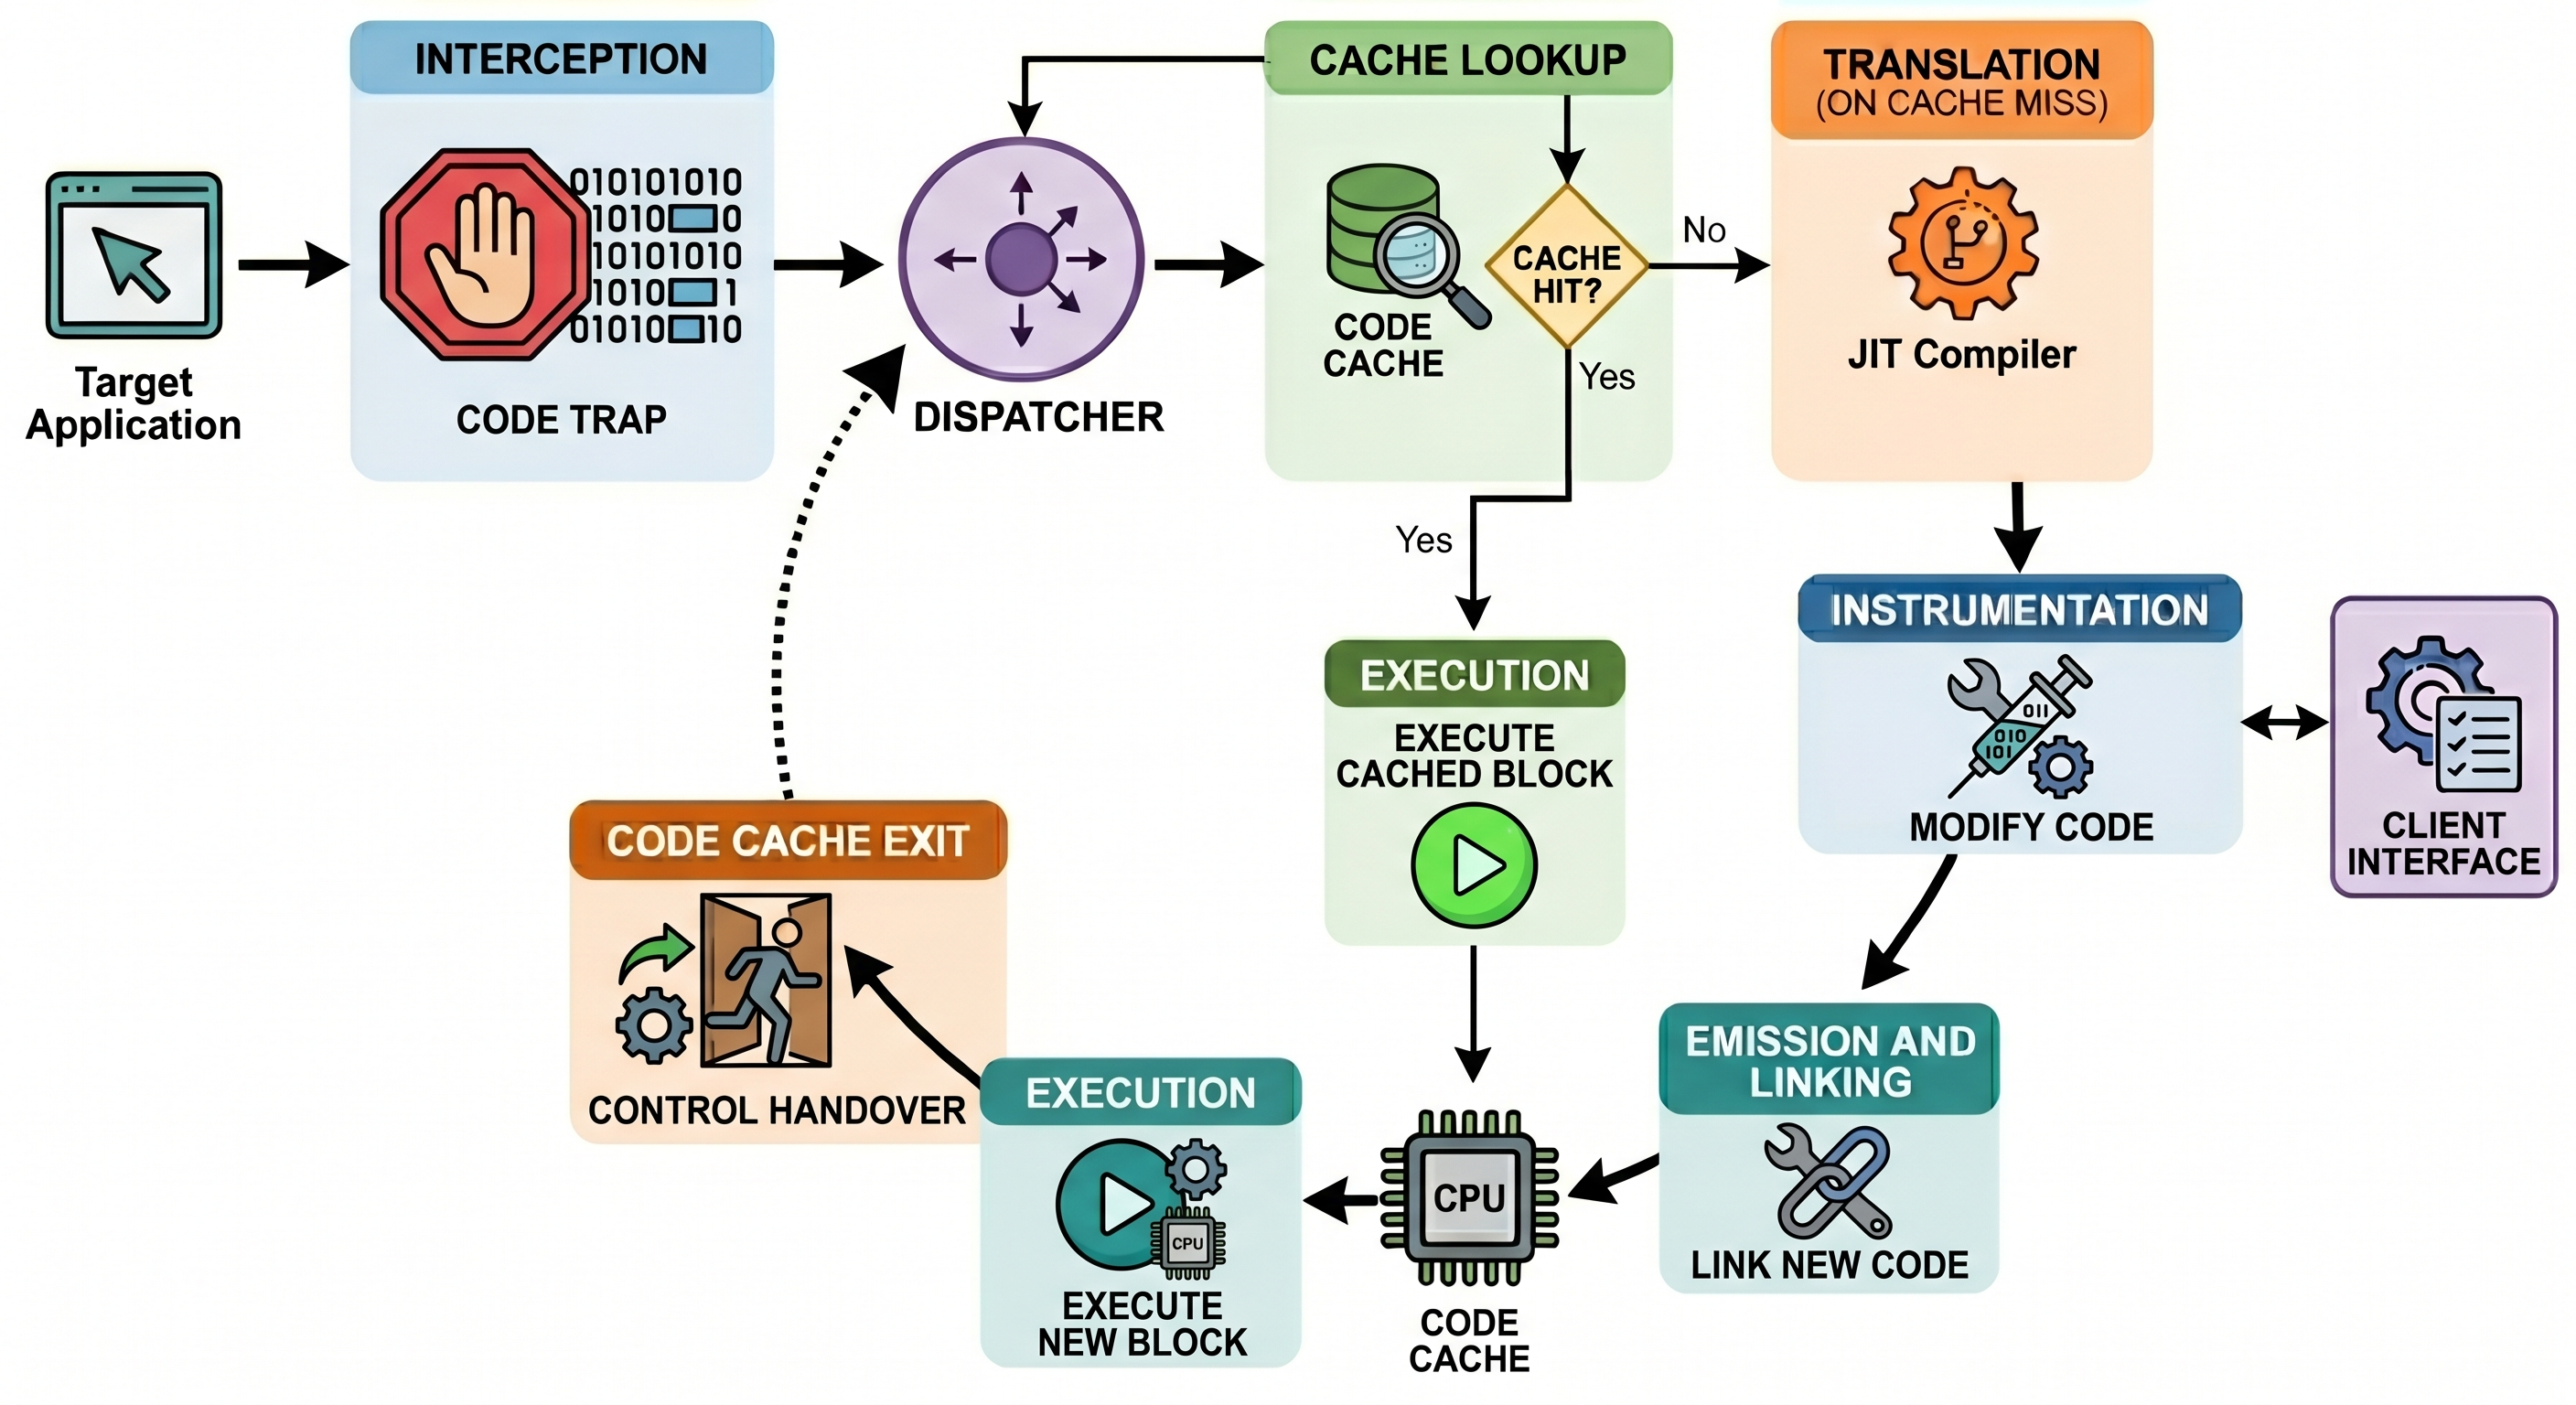
\includegraphics[width=0.9\textwidth]{images/DBI_flow.png}
	\caption{The Execution Lifecycle of a DBI framework}
	\label{fig:dbi_flow}
\end{figure}

While \ac{DBI} frameworks allow a more granular analysis of the target code, they introduce \textbf{significantly higher overhead} compared to inline hooking. Every single instruction of the program needs to be \ac{JIT}-compiled before execution, even if no instrumentation is injected.

\subsection{The Client Interface: Instrumentation vs. Analysis Functions}

\ac{DBI} frameworks require the developer to interact with the engine using a \textbf{two-tiered callback paradigm}. The developer must supply two distinct types of functions to the engine, each operating at fundamentally different times during the execution lifecycle:

\begin{itemize}
	\item \textbf{The Instrumentation Function (The ``Where'' and ``What''):} 
	This callback is invoked by the \ac{DBI} engine \emph{only once} per newly discovered sequence of instructions during the \ac{JIT} compilation phase. Its purpose is to inspect the static properties of the instructions (e.g., opcodes, operands) and decide \emph{if} and \emph{where} custom code should be injected. If injection is required, it uses the \ac{API} to queue the insertion of the analysis function.
	\item \textbf{The Analysis Function (The ``Action''):} 
	This is the actual custom payload injected into the Code Cache. Unlike the instrumentation function (executed only at compile time), it is executed \emph{every time} the CPU runs the corresponding instrumented block of code. For this reason, the analysis function must be heavily optimized and efficient.
\end{itemize}

The level of abstraction provided by the Client Interface significantly alters how developers interact with the engine.

\subsection{High-Level Abstraction: Intel PIN}
Intel PIN is a standard academic \ac{DBI} framework with a proprietary (free for non-commercial use) license. It provides a heavily abstracted C++ \ac{API}.

To utilize Intel PIN, developers do not modify the core engine itself. Instead, they write a custom C++ program known as a \emph{PINtool}. 
A PINtool represents the physical implementation of the Client Interface discussed previously; it is the user-defined module that contains both the Instrumentation Functions and the Analysis Functions. 

Architecturally, a PINtool is compiled as a standard shared library (a \ac{DLL} on Windows). When the user launches a target application under PIN, the engine automatically injects the PINtool \ac{DLL} into the target process's memory space. 
Once loaded, the engine invokes the PINtool's \texttt{main} function, allowing the tool to register its specific callbacks. 

In the following PINtool, we can observe the granularity achievable using \ac{DBI}: in this case, we can log conditional branches to determine which paths are taken during code execution.

\begin{lstlisting}[language=C++, caption={An example of a PINtool for branch logging}, label={lst:pin_branch}, basicstyle=\ttfamily\footnotesize, breaklines=true]
		// Analysis function (Runs at execution time in the Code Cache)
		void record_branch(ADDRINT instruction_address, ADDRINT target_address, BOOL taken) {
			
		  if (taken) { /* Log Taken */ } 
		  else       { /* Log Not Taken */ }
		}
		
		// Instrumentation function (Runs at JIT compilation time)
		void trace(INS instruction, void *v) {
			
		  // PIN abstracts away module resolution: we want to instrument
		  // only target application instructions, filter possible external libraries
		  RTN rtn = INS_Rtn(instruction);
		  
		  if (RTN_Valid(rtn) && IMG_IsMainExecutable(SEC_Img(RTN_Sec(rtn)))) {
		    // If it is inside the target executable, check if it's an IF branch
		    if (INS_IsBranch(instruction) && INS_HasFallThrough(instruction)) {
		      // Inject analysis function right before the jump happens.
		      INS_InsertCall(instruction, IPOINT_BEFORE, (AFUNPTR)record_branch,
		        IARG_INST_PTR,           
		        IARG_BRANCH_TARGET_ADDR,  
		        IARG_BRANCH_TAKEN,        
		        IARG_END);
		    }
		  }
		}
	\end{lstlisting}

\subsection{Bare-Metal \ac{DBI}: DynamoRIO}
DynamoRIO is the open-source alternative that exposes a lower-level C \ac{API}. 
The following code is the equivalent branch-logging example seen previously for PIN:

\begin{lstlisting}[language=C, caption={DynamoRIO branch instrumentation example}, label={lst:dr_branch}, basicstyle=\ttfamily\footnotesize, breaklines=true]
		// Analysis function
		static void record_branch(app_pc instr_addr, app_pc target_addr, int taken) {
		  
		  if (taken) { /* Log Taken */ } 
		  else       { /* Log Not Taken */ }
		}
		
		// Instrumentation function
		static dr_emit_flags_t event_bb_analysis(void *drcontext, void *tag, instrlist_t *bb, instr_t *inst, bool for_trace, bool translating,
		void *user_data) {
		  
		  // Manual module tracking to filter out OS libraries
		  app_pc instr_addr = instr_get_app_pc(inst);
		  
		  module_data_t *mod = dr_lookup_module(instr_addr);
		  bool is_main_exec = false;
		  
		  if (mod != NULL) {
		    module_data_t *main_mod = dr_get_main_module();
		    
		    if (main_mod != NULL) {
		      if (mod->start == main_mod->start) { is_main_exec = true; }
		      dr_free_module_data(main_mod);
		    }
		    dr_free_module_data(mod);
		  }
		  
		  if (!is_main_exec) return DR_EMIT_DEFAULT;
		  
		  // Check if it's a conditional branch (CBR)
		  if (instr_is_cbr(inst)) {
		    // Inject analysis function into the basic block (bb)
		    dr_insert_cbr_instrumentation(drcontext, bb, inst, (void *)record_branch);
		  }
		  return DR_EMIT_DEFAULT;
		}
	\end{lstlisting}

Using DynamoRIO, developers can directly manipulate the instruction flow. In PIN, developers generally ``wrap" existing instructions (adding a call before or after an instruction) but cannot easily modify the instruction itself. 
In DynamoRIO, the developer is handed a linked list of instructions (\texttt{instrlist\_t}) and can easily manipulate or modify them (e.g., reordering them or moving a load instruction earlier to test for race condition).

Furthermore, because PIN is designed to be highly opaque, using \texttt{INS\_InsertCall} prompts PIN's \ac{JIT} compiler to automatically analyze the custom analysis function for deciding which registers need to be saved and restored based on what the C++ code actually uses. 
With DynamoRIO, developers can manage the state and flags manually for specialized analysis.

In conclusion, while DynamoRIO may present a steeper learning curve than Intel PIN, it affords developers greater transparency and raw power, providing fine-grained control over the translated code and the code cache.